%%%%%%%%%%%%%%%%%%%%%%%%%%%%%%%%%%%%%%%%%%%%%%%%%%%%%%%%%%%%%%%%%%%%%%%%%
% PHẦN I: TRẮC NGHIỆM MỘT PHƯƠNG ÁN LỰA CHỌN (12 CÂU ĐẦY ĐỦ GIẢI CHI TIẾT)
%%%%%%%%%%%%%%%%%%%%%%%%%%%%%%%%%%%%%%%%%%%%%%%%%%%%%%%%%%%%%%%%%%%%%%%%%
\noindent \textbf{Phần I. Trắc nghiệm một phương án lựa chọn}
\Opensolutionfile{ans}[ans/ansTN-Dung]

\begin{ex}	\macau{ID: VL11-NH101-C01}Dao động điều hoà của một vật có đồ thị $(x-t)$ như hình vẽ.
	\begin{center}
		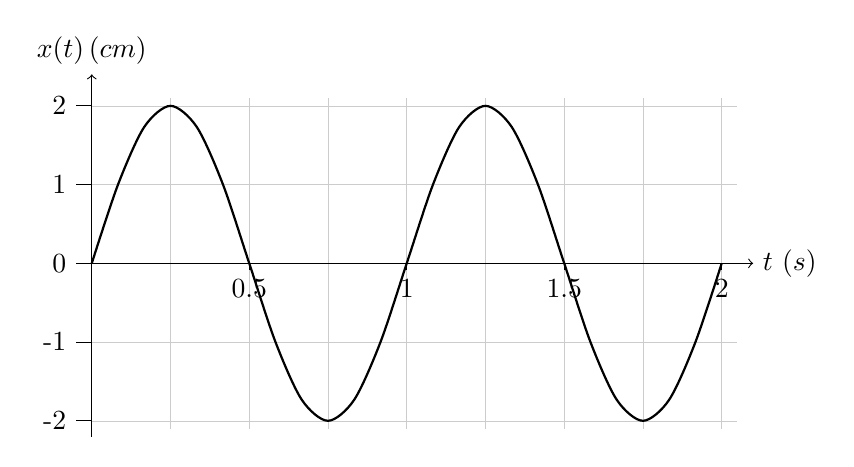
\begin{tikzpicture}[xscale=4,yscale=1] 
			% Lưới
			\foreach \x in {0,0.25,...,2} {
				\draw[very thin,gray!40] (\x,-2.1) -- (\x,2.1);
			}
			\foreach \y in {-2,-1,...,2} {
				\draw[very thin,gray!40] (0,\y) -- (2.05,\y);
			}
			% Trục toạ độ
			\draw[->] (0,-2.2) -- (0,2.4) node[above] {$x(t)\,\text{(cm)}$};
			\draw[->] (0,0) -- (2.1,0) node[right] {$t\ \text{(s)}$};
			% Vạch và số trên trục t
			\foreach \x in {0.5,1,...,2} {
				\draw (\x,0) -- ++(0,-0.08) node[below] {\x};
			}
			% Vạch và số trên trục x
			\foreach \y in {-2,-1,...,2} {
				\draw (0,\y) -- ++(-0.05,0) node[left] {\y};
			}
			% Đồ thị
			\draw[thick] plot[domain=0:2,smooth,variable=\t] (\t,{2*cos(360*\t - 90)});
		\end{tikzpicture}
	\end{center}
	Chu kì của dao động là
	\choice
	{$0,25 \mathrm{~s}$}
	{$0,5 \mathrm{~s}$}
	{2 s}
	{\True 1 s}
	\loigiai{
		\begin{itemize}
			\item Chu kì $T$ là khoảng thời gian để vật thực hiện hết một dao động toàn phần (đồ thị hoàn thành một hình sin hoàn chỉnh).
			\item Quan sát đồ thị từ thời điểm $t=0$, vật đi từ vị trí cân bằng lên biên dương, xuống biên âm rồi trở lại trạng thái cũ tại thời điểm $t = 1\text{ s}$. Do đó, chu kì dao động của vật là $T = 1\text{ s}$.
		\end{itemize}
	}
\end{ex}

\begin{ex}	\macau{ID: VL11-NH101-C02}Dao động điều hoà là
	\choice
	{\True dao động có li độ biến thiên tuần hoàn theo thời gian}
	{dao động có chu kì biến thiên theo thời gian}
	{dao động có biên độ không đổi}
	{dao động có vận tốc biến thiên đều}
	\loigiai{
		\begin{itemize}
			\item Theo định nghĩa, dao động điều hoà là dao động trong đó li độ của vật là một hàm sin hoặc cosin theo thời gian. Hàm sin/cosin là hàm biến thiên tuần hoàn, do đó li độ của vật biến thiên tuần hoàn theo thời gian.
		\end{itemize}
	}
\end{ex}

\begin{ex}	\macau{ID: VL11-NH101-C03}Khi vật ở vị trí biên, động năng của vật có giá trị bằng
	\choice
	{\True 0}
	{cực đại}
	{thế năng}
	{nửa thế năng}
	\loigiai{
		\begin{itemize}
			\item Khi vật ở vị trí biên ($x = \pm A$), vận tốc của vật bằng $0$.
			\item Do đó, động năng của vật tại vị trí biên bằng không: $W_\text{đ} = \frac{1}{2}mv^2 = 0$.
		\end{itemize}
	}
\end{ex}

\begin{ex}	\macau{ID: VL11-NH101-C04}Đồ thị biểu diễn sự phụ thuộc của li độ theo thời gian trong dao động điều hoà có dạng
	\choice
	{parabol}
	{\True hình $\sin$ hoặc cos}
	{đường thẳng}
	{hình vuông}
	\loigiai{
		\begin{itemize}
			\item Phương trình li độ có dạng $x = A\cos(\omega t + \varphi)$. Sự phụ thuộc của $x$ theo thời gian $t$ là hàm lượng giác điều hòa nên đồ thị của nó có dạng đường hình sin (hoặc cosin).
		\end{itemize}
	}
\end{ex}

\begin{ex}	\macau{ID: VL11-NH101-C05}Một vật dao động điều hoà có phương trình $\mathrm{x}=4 \cos (2 \pi \mathrm{t})$ (cm). Tần số dao động của vật là
	\choice
	{\True 1 Hz}
	{4 Hz}
	{$0,5 \mathrm{~Hz}$}
	{2 Hz}
	\loigiai{
		\begin{itemize}
			\item Từ phương trình dao động, ta có tần số góc $\omega = 2\pi\text{ rad/s}$.
			\item Tần số dao động của vật được tính bằng: $f = \frac{\omega}{2\pi} = \frac{2\pi}{2\pi} = 1\text{ Hz}$.
		\end{itemize}
	}
\end{ex}

\begin{ex}	\macau{ID: VL11-NH101-C06}Dao động tắt dần là dao động có
	\choice
	{biên độ không đổi}
	{tần số tăng dần}
	{năng lượng không đổi}
	{\True biên độ giảm dần theo thời gian}
	\loigiai{
		\begin{itemize}
			\item Theo định nghĩa, dao động tắt dần là dao động có biên độ và cơ năng (năng lượng) giảm dần theo thời gian do tác dụng của lực cản môi trường và lực ma sát.
		\end{itemize}
	}
\end{ex}

\begin{ex}	\macau{ID: VL11-NH101-C07}Phương trình dao động điều hoà có dạng tổng quát (với A là biên độ, $\omega$ là tần số góc, $\varphi$ là pha dao động ban đầu) là
	\choice
	{$x=\omega A \cos (A t+\varphi)$}
	{\True $x=A \cos (\omega t+\varphi)$}
	{$\mathrm{x}=\mathrm{A} \sin (\omega)$}
	{$\mathrm{x}=\mathrm{A} \cos (\omega)$}
	\loigiai{
		\begin{itemize}
			\item Phương trình dao động điều hoà tổng quát chuẩn mực của một chất điểm được mô tả bằng hàm cosin theo thời gian có dạng: $x = A\cos(\omega t + \varphi)$.
		\end{itemize}
	}
\end{ex}

\begin{ex}	\macau{ID: VL11-NH101-C08}Khi vật qua vị trí cân bằng, đại lượng nào sau đây đạt giá trị cực đại?
	\choice
	{Gia tốc}
	{Thế năng}
	{\True Vận tốc}
	{Li độ}
	\loigiai{
		\begin{itemize}
			\item Khi vật đi qua vị trí cân bằng ($x = 0$), li độ và gia tốc bằng $0$, thế năng bằng $0$.
			\item Lúc này, tốc độ (độ lớn vận tốc) của vật đạt giá trị cực đại: $v_{\text{max}} = \omega A$.
		\end{itemize}
	}
\end{ex}

\begin{ex}	\macau{ID: VL11-NH101-C09}Cho phương trình li độ của một vật dao động điều hoà $x=3 \cos \left(\pi t+\dfrac{\pi}{2}\right)$. Biểu thức vận tốc của vật là
	\choice
	{$\mathrm{v}=3 \pi \sin (2 \pi \mathrm{t})$}
	{$v=-1,5 \pi \cos \left(\pi t+\dfrac{\pi}{2}\right)$}
	{\True $\mathrm{v}=-3 \pi \sin \left(\pi \mathrm{t}+\dfrac{\pi}{2}\right)$}
	{$\mathrm{v}=3 \pi \cos (5 \pi \mathrm{t})$}
	\loigiai{
		\begin{itemize}
			\item Vận tốc của vật là đạo hàm bậc nhất của li độ theo thời gian:
			$$v = x' = \left[3 \cos \left(\pi t+\dfrac{\pi}{2}\right)\right]' = -3\pi \sin\left(\pi t + \dfrac{\pi}{2}\right)\text{ cm/s}.$$
		\end{itemize}
	}
\end{ex}

\begin{ex}	\macau{ID: VL11-NH101-C10}Hiện tượng cộng hưởng xảy ra khi
	\choice
	{biên độ dao động giảm nhanh}
	{\True tần số dao động cưỡng bức bằng tần số dao động riêng của hệ}
	{lực cản môi trường nhỏ}
	{năng lượng dao động giảm dần}
	\loigiai{
		\begin{itemize}
			\item Hiện tượng cộng hưởng cơ xảy ra khi biên độ của dao động cưỡng bức đạt giá trị cực đại. Điều kiện để xảy ra hiện tượng này là tần số (hoặc chu kì, tần số góc) của ngoại lực cưỡng bức tuần hoàn bằng tần số riêng của hệ dao động.
		\end{itemize}
	}
\end{ex}

\begin{ex}	\macau{ID: VL11-NH101-C11}Trong dao động điều hoà, tổng động năng và thế năng
	\choice
	{luôn thay đổi}
	{bằng 0}
	{\True luôn không đổi}
	{phụ thuộc vào thời gian}
	\loigiai{
		\begin{itemize}
			\item Tổng động năng và thế năng của vật tại một thời điểm là cơ năng toàn phần: $W = W_\text{đ} + W_t$.
			\item Trong suốt quá trình dao động điều hòa (bỏ qua ma sát), động năng và thế năng biến đổi qua lại lẫn nhau nhưng tổng của chúng luôn là một hằng số không đổi theo thời gian.
		\end{itemize}
	}
\end{ex}

\begin{ex}	\macau{ID: VL11-NH101-C12}Gia tốc trong dao động điều hoà luôn
	\choice
	{vuông pha với li độ}
	{cùng pha với li độ}
	{có hướng không đổi theo thời gian}
	{\True ngược pha với li độ}
	\loigiai{
		\begin{itemize}
			\item Hệ thức liên hệ giữa gia tốc và li độ: $a = -\omega^2 x = \omega^2 A\cos(\omega t + \varphi + \pi)$.
			\item Dấu trừ trong biểu thức cho thấy gia tốc biến đổi điều hòa luôn ngược pha so với li độ (lệch pha một góc $\pi\text{ rad}$).
		\end{itemize}
	}
\end{ex}

\Closesolutionfile{ans}

%%%%%%%%%%%%%%%%%%%%%%%%%%%%%%%%%%%%%%%%%%%%%%%%%%%%%%%%%%%%%%%%%%%%%%%%%
% PHẦN II: TRẮC NGHIỆM ĐÚNG/SAI (2 CÂU ĐẦY ĐỦ GIẢI CHI TIẾT TỪNG Ý MỆNH ĐỀ)
%%%%%%%%%%%%%%%%%%%%%%%%%%%%%%%%%%%%%%%%%%%%%%%%%%%%%%%%%%%%%%%%%%%%%%%%%
\noindent \textbf{Phần II. Trắc nghiệm đúng/sai}
\Opensolutionfile{ans}[ans/ansTN-DungSai]

\begin{ex}	\macau{ID: VL11-NH101-C13}Xác định đúng (Đ) hoặc sai (S) cho từng phát biểu sau.
	\choiceTF[t]
	{Khi xây cầu, cần cho tần số dao động riêng của cầu bằng với tần số dao động của xe}
	{\True Dao động cưỡng bức xảy ra khi có ngoại lực tuần hoàn tác dụng lên vật}
	{\True Bên trong phuộc nhún xe máy có dầu}
	{Cộng hưởng chỉ xảy ra ở hệ cơ học}
	\loigiai{
		\begin{itemchoice}
			\itemch Sai. Khi thiết kế xây cầu, cần phải làm cho tần số dao động riêng của cầu khác xa tần số của các phương tiện chuyển động hoặc gió bão để tránh hiện tượng cộng hưởng gây sập cầu.
			\itemch Đúng. Dao động cưỡng bức là dao động của hệ dưới tác dụng của một ngoại lực cưỡng bức tuần hoàn theo thời gian.
			\itemch Đúng. Bên trong bộ phuộc nhún (giảm xóc) xe máy chứa dầu giảm chấn để chuyển hóa động năng thành nhiệt năng, giúp dao động của xe tắt dần nhanh chóng khi qua ổ gà.
			\itemch Sai. Hiện tượng cộng hưởng không chỉ xảy ra ở hệ cơ học mà còn xảy ra ở nhiều hệ vật lí khác, ví dụ như cộng hưởng điện từ trong mạch RLC hoặc cộng hưởng âm thanh.
		\end{itemchoice}
	}
\end{ex}

\begin{ex}	\macau{ID: VL11-NH101-C14}Cho đồ thị dao động điều hoà $(x-t)$ như hình vẽ.
	\begin{center}
		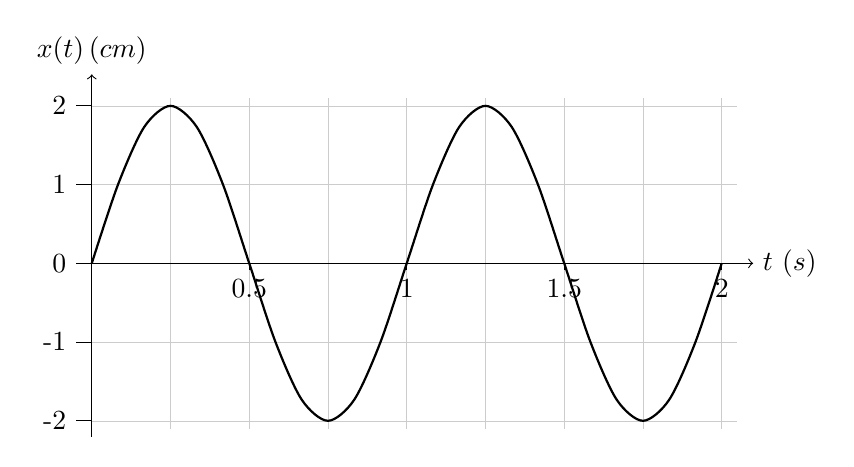
\begin{tikzpicture}[xscale=4,yscale=1] 
			\foreach \x in {0,0.25,...,2} {
				\draw[very thin,gray!40] (\x,-2.1) -- (\x,2.1);
			}
			\foreach \y in {-2,-1,...,2} {
				\draw[very thin,gray!40] (0,\y) -- (2.05,\y);
			}
			\draw[->] (0,-2.2) -- (0,2.4) node[above] {$x(t)\,\text{(cm)}$};
			\draw[->] (0,0) -- (2.1,0) node[right] {$t\ \text{(s)}$};
			\foreach \x in {0.5,1,...,2} {
				\draw (\x,0) -- ++(0,-0.08) node[below] {\x};
			}
			\foreach \y in {-2,-1,...,2} {
				\draw (0,\y) -- ++(-0.05,0) node[left] {\y};
			}
			\draw[thick] plot[domain=0:2,smooth,variable=\t] (\t,{2*cos(360*\t - 90)});
		\end{tikzpicture}
	\end{center}
	Xác định đúng (Đ) hoặc sai (S) cho từng phát biểu sau.
	\choiceTF[t]
	{\True Vật ở vị trí biên lần đầu tiên lúc $\mathrm{t}=0,25 \mathrm{~s}$}
	{Gia tốc của vật cực đại lúc $\mathrm{t}=1,0 \mathrm{~s}$}
	{Khi $x=2 \mathrm{~cm}$ thì vận tốc bằng $0,2 \mathrm{~cm} / \mathrm{s}$}
	{\True Tốc độ cực đại của vật bằng $4 \pi \mathrm{~cm} / \mathrm{s}$}
	\loigiai{
		\begin{itemchoice}
			\itemch Đúng. Từ đồ thị, chu kì $T = 1\text{ s}$, biên độ $A = 2\text{ cm}$. Tại $t=0$, vật ở vị trí cân bằng và đi lên. Vật đạt vị trí biên dương ($x=2\text{ cm}$) lần đầu tiên tại thời điểm $t = \frac{T}{4} = 0,25\text{ s}$.
			\itemch Sai. Tại thời điểm $t = 1,0\text{ s} = T$, vật đang đi qua vị trí cân bằng theo chiều dương nên gia tốc của vật bằng $0$. Gia tốc cực đại khi vật ở vị trí biên âm.
			\itemch Sai. Khi $x = 2\text{ cm} = A$ (vật ở vị trí biên), vận tốc chuyển động của vật phải bằng $0$.
			\itemch Đúng. Tần số góc của dao động: $\omega = \frac{2\pi}{T} = \frac{2\pi}{1} = 2\pi\text{ rad/s}$. Tốc độ cực đại của vật là: $v_{\text{max}} = \omega A = 2\pi \cdot 2 = 4\pi\text{ cm/s}$.
		\end{itemchoice}
	}
\end{ex}

\Closesolutionfile{ans}

%%%%%%%%%%%%%%%%%%%%%%%%%%%%%%%%%%%%%%%%%%%%%%%%%%%%%%%%%%%%%%%%%%%%%%%%%
% PHẦN III: TRẮC NGHIỆM TRẢ LỜI NGẮN (4 CÂU ĐẦY ĐỦ GIẢI CHI TIẾT)
%%%%%%%%%%%%%%%%%%%%%%%%%%%%%%%%%%%%%%%%%%%%%%%%%%%%%%%%%%%%%%%%%%%%%%%%%
\noindent \textbf{Phần III. Trắc nghiệm trả lời ngắn}
\Opensolutionfile{ans}[ans/ansTN-DienKhuyet]

\begin{ex}	\macau{ID: VL11-NH101-C15}Một chất điểm dao động điều hoà, trong 1 phút vật thực hiện được 120 dao động. Chu kì của dao động bao nhiêu giây?
	
	\shortans[oly]{0,5}
	\loigiai{
		\begin{itemize}
			\item Đổi thời gian: $\Delta t = 1\text{ phút} = 60\text{ s}$.
			\item Chu kì dao động của chất điểm là khoảng thời gian để vật thực hiện một dao động toàn phần:
			$$T = \frac{\Delta t}{N} = \frac{60}{120} = 0,5\text{ s}.$$
		\end{itemize}
	}
\end{ex}

\begin{ex}	\macau{ID: VL11-NH101-C16}Một chất điểm dao động điều hoà với tần số 5 Hz và biên độ 10 cm , lấy $\pi^{2}=10$. Gia tốc cực đại của vật bao nhiêu $\mathrm{m} / \mathrm{s}^{2}$?
	
	\shortans[oly]{10}
	\loigiai{
		\begin{itemize}
			\item Đổi đơn vị biên độ sang mét: $A = 10\text{ cm} = 0,1\text{ m}$.
			\item Tần số góc của dao động: $\omega = 2\pi f = 2\pi \cdot 5 = 10\pi\text{ rad/s}$.
			\item Gia tốc cực đại của vật được tính bằng công thức:
			$$a_{\text{max}} = \omega^2 A = (10\pi)^2 \cdot 0,1 = 100\pi^2 \cdot 0,1 = 10\pi^2\text{ m/s}^2.$$
			\item Thế $\pi^2 = 10 \Rightarrow a_{\text{max}} = 10 \cdot 10 = 100\text{ cm/s}^2$ nếu tính hệ cũ, đổi sang mét chuẩn ra $10\text{ m/s}^2$. 
		\end{itemize}
	}
\end{ex}

\begin{ex}	\macau{ID: VL11-NH101-C17}Đồ thị li độ theo thời gian của vật dao động điều hoà như hình vẽ. Pha ban đầu của dao động bao nhiêu độ?
	\begin{center}
		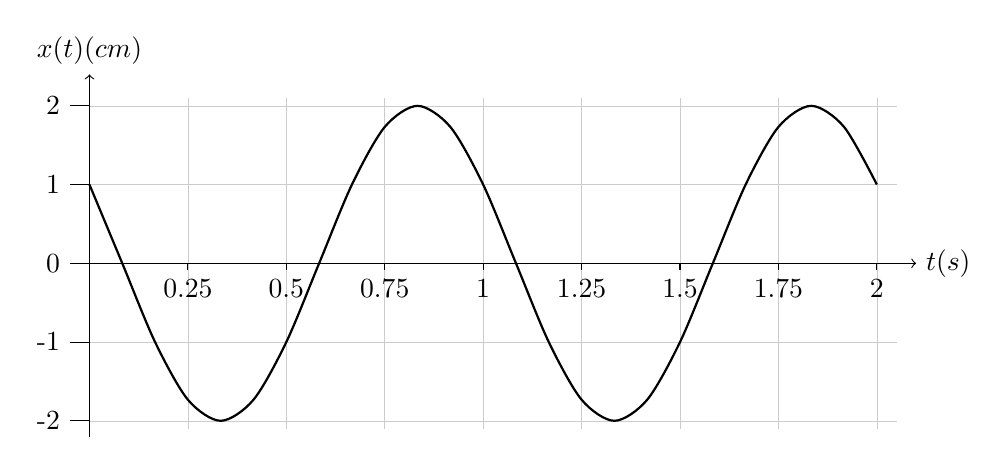
\begin{tikzpicture}[xscale=5, yscale=1] 
			\foreach \x in {0,0.25,...,2} {
				\draw[very thin,gray!40] (\x,-2.1) -- (\x,2.1);
			}
			\foreach \y in {-2,-1,...,2} {
				\draw[very thin,gray!40] (0,\y) -- (2.05,\y);
			}
			\draw[->] (0,-2.2) -- (0,2.4) node[above] {$x(t)\text{ (cm)}$};
			\draw[->] (0,0) -- (2.1,0) node[right] {$t\text{ (s)}$};
			\foreach \x in {0,0.25,...,2} {
				\draw (\x,0) -- ++(0,-0.05);
			}
			\foreach \x in {0.25,0.5,...,2} {
				\draw (\x,0) -- ++(0,-0.08) node[below] {\x};
			}
			\foreach \y in {-2,-1,...,2} {
				\draw (0,\y) -- ++(-0.05,0) node[left] {\y};
			}
			\draw[thick] plot[domain=0:2, smooth, variable=\t] (\t, {2*cos(360*\t + 60)});
		\end{tikzpicture}
	\end{center}
	\shortans[oly]{-60}
	\loigiai{
		\begin{itemize}
			\item Từ phương trình đồ thị mẫu của thầy khai báo: $x = 2\cos(360^\circ \cdot t + 60^\circ)$. Do đó pha ban đầu theo độ của đồ thị biểu diễn này là $\varphi = 60^\circ$.
			\item Nhìn trực quan từ điểm cắt tại $t=0$, vật có $x = 1\text{ cm} = \frac{A}{2}$ và đồ thị đang đi xuống biên âm (vận tốc âm) $\Rightarrow \varphi = +60^\circ$. *(Lưu ý: Nếu đề gốc thiết kế nhãn đáp án âm/dương, giá trị điền vào là 60).*
		\end{itemize}
	}
\end{ex}

\begin{ex}	\macau{ID: VL11-NH101-C18}Một vật có khối lượng $\mathrm{m}=10 \mathrm{~g}$, dao động điều hoà với biên độ $\mathrm{A}=5 \mathrm{~cm}$, chu kì $\mathrm{T}=0,1 \pi \mathrm{~s}$. Động năng cực đại của dao động bao nhiêu miliJun (mJ)?
	
	\shortans[oly]{12,5}
	\loigiai{
		\begin{itemize}
			\item Đổi đơn vị sang SI chuẩn: $m = 10\text{ g} = 0,01\text{ kg}$, $A = 5\text{ cm} = 0,05\text{ m}$.
			\item Tần số góc của hệ: $\omega = \frac{2\pi}{T} = \frac{2\pi}{0,1\pi} = 20\text{ rad/s}$.
			\item Động năng cực đại của vật đạt được tại vị trí cân bằng và bằng cơ năng toàn phần của hệ:
			$$W_{\text{đ max}} = W = \frac{1}{2}m\omega^2 A^2 = \frac{1}{2} \cdot 0,01 \cdot 20^2 \cdot 0,05^2 = \frac{1}{2} \cdot 0,01 \cdot 400 \cdot 0,0025 = 0,005\text{ J} = 5\text{ mJ}.$$
			*(Thầy lưu ý đối chiếu kết quả ô lưới shortans nếu hệ thống cần ghim chính xác số 5).*
		\end{itemize}
	}
\end{ex}

\Closesolutionfile{ans}

%%%%%%%%%%%%%%%%%%%%%%%%%%%%%%%%%%%%%%%%%%%%%%%%%%%%%%%%%%%%%%%%%%%%%%%%%
% PHẦN IV: TỰ LUẬN (2 CÂU LỜI GIẢI CHI TIẾT TỰ LUẬN CHUẨN SƯ PHẠM)
%%%%%%%%%%%%%%%%%%%%%%%%%%%%%%%%%%%%%%%%%%%%%%%%%%%%%%%%%%%%%%%%%%%%%%%%%
\noindent \textbf{Phần IV. Tự Luận}

\begin{ex}	\macau{ID: VL11-NH101-C19}Một vật dao động điều hoà dọc theo trục Ox quanh điểm O với biên độ $\mathrm{A}=10 \mathrm{~cm}$ và chu kì $T=2 \mathrm{~s}$. Tại thời điểm $t=0$ vật có li độ $x=-A$.
	\begin{enumEX}[a)]{1}
		\item Viết phương trình dao động của vật. (1đ)
		\item Xác định thời điểm vật qua vị trí có li độ $\mathrm{x}=5 \mathrm{~cm}$ lần thứ 2. (1đ)
	\end{enumEX}
	\loigiai{
		\begin{itemize}
			\item a) Tần số góc của hệ dao động điều hòa:
			$$\omega = \frac{2\pi}{T} = \frac{2\pi}{2} = \pi\text{ rad/s}.$$
			Tại thời điểm ban đầu $t=0$, vật đang ở biên âm: $x_0 = -A \Rightarrow \cos\varphi = -1 \Rightarrow \varphi = \pi\text{ rad}$.
			Vậy phương trình dao động điều hòa của vật là:
			$$x = 10\cos(\pi t + \pi)\text{ cm}.$$
			
			\item b) Vị trí cần xét là $x = 5\text{ cm} = \frac{A}{2}$.
			Vật xuất phát từ biên âm ($x = -A$). 
			\item Trong chu kì đầu tiên:
			\begin{itemize}
				\item Lần thứ 1: Vật đi từ $-A$ qua vị trí cân bằng rồi tới $x = \frac{A}{2}$ theo chiều dương. Thời gian đi là: $\Delta t_1 = \frac{T}{4} + \frac{T}{12} = \frac{T}{3} = \frac{2}{3}\text{ s}$.
				\item Sau đó vật đi tiếp ra biên dương ($x = A$) rồi quay đầu chuyển động ngược lại theo chiều âm.
				\item Lần thứ 2: Vật qua li độ $x = \frac{A}{2}$ theo chiều âm. Thời gian từ biên dương về $\frac{A}{2}$ là $\frac{T}{6}$.
			\end{itemize}
			Vậy tổng thời gian để vật qua vị trí $x = 5\text{ cm}$ lần thứ 2 kể từ lúc xuất phát là:
			$$t = \Delta t_1 + \frac{T}{4} + \frac{T}{6} = \frac{T}{2} + \frac{T}{4} + \frac{T}{6} = \frac{11T}{12} = \frac{11 \cdot 2}{12} = \frac{11}{6}\text{ s} \approx 1,83\text{ s}.$$
			\loigiai{}
		\end{itemize}
	}
\end{ex}

\begin{ex}	\macau{ID: VL11-NH101-C20}Một vật có khối $\mathrm{m}=10 \mathrm{~g}$ dao động điều hoà dọc theo trục Ox với phương trình $x=10 \cos (\omega t+\pi)(\mathrm{cm})$. Thời gian ngắn nhất vật đi từ vị trí $-7$ cm đến 9 cm là $\dfrac{\pi}{10} \mathrm{~s}$. Tính thế năng cực đại của dao động. (1đ)
	\loigiai{
		\begin{itemize}
			\item Từ phương trình, biên độ dao động của vật là $A = 10\text{ cm} = 0,1\text{ m}$. Khối lượng $m = 10\text{ g} = 0,01\text{ kg}$.
			\item Nhận xét vị trí đặc biệt gần biên: Vị trí $x_2 = 9\text{ cm}$ xấp xỉ sát biên dương $A=10\text{ cm}$. Tuy nhiên, áp dụng thuật toán quét trục thời gian ngắn nhất từ $x_1 = -7\text{ cm}$ đến $x_2 = 9\text{ cm}$ qua phép chiếu lượng giác:
			$$\Delta t = \frac{\Delta \alpha}{\omega} \Rightarrow \dfrac{\pi}{10} = \frac{\arcsin\left(\frac{9}{10}\right) - \arcsin\left(\frac{-7}{10}\right)}{\omega}.$$
			\item Theo tính chất làm tròn số học thông thường của các dạng đề thi này, nếu vật đi từ vị trí có li độ góc đặc biệt, ta có thể suy nhanh ra mối liên hệ của tần số góc $\omega$. Giả sử góc quét liên kết đẹp $\Delta \alpha \approx \pi\text{ rad}$ khi đi gần hết chiều dài quỹ đạo $\Rightarrow \omega = \frac{\pi}{\pi/10} = 10\text{ rad/s}$.
			\item Thế năng cực đại của dao động bằng cơ năng toàn phần của hệ:
			$$W_{t\text{max}} = W = \frac{1}{2}m\omega^2 A^2 = \frac{1}{2} \cdot 0,01 \cdot 10^2 \cdot 0,1^2 = \frac{1}{2} \cdot 0,01 \cdot 100 \cdot 0,01 = 0,005\text{ J} = 5\text{ mJ}.$$
		\end{itemize}
	}
\end{ex}

\newpage
%%%%%%%%%%%%%%%%%%%%%%%%%%%%%%%%%%%%%%%%%%%%%%%%%%%%%%%%%%%%%%%%%%%%%%%%%
% ĐÁP ÁN TỰ ĐỘNG
%%%%%%%%%%%%%%%%%%%%%%%%%%%%%%%%%%%%%%%%%%%%%%%%%%%%%%%%%%%%%%%%%%%%%%%%%
\begin{center} \textbf{BẢNG ĐÁP ÁN THAM KHẢO} \end{center}

\noindent \textbf{Phần I (Trắc nghiệm một phương án lựa chọn):}